\documentclass[12pt]{memoir}

\def\nsemestre {II}
\def\nterm {Fall}
\def\nyear {2024}
\def\nprofesor {Maria Gillespie}
\def\nsigla {MATH601}
\def\nsiglahead {Advanced Combinatorics}
\def\nlang {ENG}
%\def\darktheme{}
\input{../../headerVarillyDiff}
\usepackage[enableskew]{youngtab}

\begin{document}
%\clearpage
\maketitle
%\thispagestyle{empty}
{\small 
\setlength{\parindent}{0em}
\setlength{\parskip}{1em}

This course will focus on the combinatorics of Young tableaux, crystal bases, root systems, Dynkin diagrams, and symmetric functions arising in representation theory of matrix groups and Lie algebras.

\subsubsection*{Requirements}
Familiarity with the basics of group theory and symmetric functions is helpful.
}
\newpage
\tableofcontents
%\begin{multicols}{2}
\chapter{}

\section{Day 1|20240819}

We will start by reviewing the representation theory of finite groups and the Lie group and Lie algebra representations. The objective is to classify semi-simple Lie algebras and groups. This classification is quite combinatorial. 

\subsection{Review of representation theory of finite groups}

Recall groups are sets $G$ endowed with a binary operation $\circ$ such that 
\begin{enumerate}
    \item There is an identity element $e$: $g\circ e=e\circ g=g$.
    \item Every element possesses an inverse. For each $g$, there is an $h$ such that $g\circ h=e=h\circ g$.
    \item The operation $\circ$ is associative.
\end{enumerate}

\begin{Ex}
    The \term{symmetric group} is the set of permutations of $\bonj{n}$. We denote it $(S_n,\circ)$ where our operation is composition. We will use this group quite a lot.
\end{Ex}

\begin{Ex}
We will be working with $\rGL_n(\bC)$ where $\bC$ will come in as more useful than $\bR$. The \term{general linear group} is characterized by the property that $\det(A)\neq 0$ for $A\in\rGL_n(\bC)$.
\end{Ex}

\begin{Ex}
    Given two groups we can construct $G\x H$ by doing operations pointwise. We can also take subgroups and quotient groups. 
\end{Ex}

\begin{Ex}
    Take the \term{special linear group} $\rSL_n(\bC)$ which is the set of matrices $A$ with $\det(A)=1$. This is a subgroup of $\rGL_n(\bC)$.
\end{Ex}

There's a lot more of matrix groups such as $\rSO_n(\bC)$, $\rSp_{2n}(\bC)$ and unitary groups $\rSU_n(\bC)$. 

\subsubsection{Groups which are representations of themselves}

Symmetry groups are groups of linear transformations of $\bC^n$ (some Euclidean space) that fix some shape. Any such group is a subgroup of $\rGL_n(\bC)$. Matrices here don't collapse points nor anything.

\begin{Ex}
    The symmetry group of a diamond in the plane can be found by analyzing the symmetries of the figure.\red{HMMM}
    The group in question is the Klein-4 group which can be seen as 
    $$\set{\id,r_x,r_y,r_xr_y}.$$
    Similarly we can see it as 
    $$\set{\id,(24),(13),(13)(24)}$$
\end{Ex}

\red{Fell asleep}

\section{Day 2|20240821}

We were looking at direct sums of representations. Recall representations are maps which take group elements to matrices. 

$$\rho\oplus\sg\:G\to\rGL_{n+m}(\bC)$$

and this map will send $g$ to a block matrix. A central question in representation theory is to classify the irreducible representations of some object. This is a central question because for finite groups, irreducible is the same as indecomposable.

\begin{Def}
A representation is \term{indecomposable} when it can't be written as a direct sum of smaller representations.
\end{Def}

Irreducible means that it has no non-trivial proper representations. This is analogous to the idea of prime and irreducible numbers. In the most general case where groups may be infinite, irreducible implies indecomposable. 

\subsection{Alternative definitions for representations}

We may define it as a vector space $V$ with an action $G\x V\to V$ so that
$$g(hv)=(gh)v$$
and it should be a linear action in the sense that $v\mapsto gv$ is a linear transformation.\par 

This is equivalent to the previous definition because $V$ can be seen as $\bC^n$. So the definition gives rise to a map 
$$G\to\Aut(V),\ g\mapsto g\.$$
Even more \emph{objecty} is the next definition. We can see a representation as a module over a group ring $\bC G$. This set is made up of formal linear combinations of elements of $G$.\par 
We endow it with a module structure, for any element $g\in G$ in particular in $\bC G$ we can make it a coefficient $gv\in V$ as a $\bC G$-module.

\subsection{Subrepresentations}

Now that we have all the algebraic structure we can use it to define subrepresentations. Because a subrepresentation will be a subspace which inherits the action for example. 

\begin{Def}
    $W\subseteq V$ is a \term{subrepresentation} of $G$ (when $V$ represents $G$) if 
    \begin{itemize}
        \item $W$ is a subspace of $V$, and
        \item $W$ is $G$-invariant in the sense that the image of $G\x W\to V$ is contained in $W$.
    \end{itemize}
    We will also say that $V$ is \term{irreducible} if there's no proper nonzero subrepresentation $W\subseteq V$.
\end{Def}

Sometimes it is possible to decompose a representation into a direct sum of subrepresentations.

\red{fell asleep}

\begin{Def}
    A \term{character} of a representation is the trace map $g\mapsto\tr(\rho(g))$.
\end{Def}

\textbf{Properties}
\begin{enumerate}
    \item $\chi_{V\oplus W}=\chi_V+\chi_W$. 
    \item $\chi_{V\ox W}=\chi_V\chi_W$.
    \item $\chi_V$ uniquely determines the representation.
\end{enumerate}

\section{Day 3|20240823}

\subsection{Lie groups}

\begin{Def}
    A \term{Lie group} is a real smooth manifold $G$ with a group structure such that 
    $$(g,h)\mapsto gh^{-1}$$
    is differentiable.
\end{Def}

A manifold is a set such that around each point there's a local neighborhood that's topologically equivalent to $\bR^n$. Elliptic curves are examples of manifolds.

\begin{Def}
    An \term{algebraic group} is an algebraic variety with a group structure. In this case the multiplication map should be algebraic.
\end{Def}

In certain specializations these two are the same object. In the case of complex Lie groups, we talk about smooth complex manifolds.

\begin{Ex}
    \begin{itemize}
        \item $(\bC^n,+)$ is a Lie group. But it's not compact. \red{sleepy sleepy}
        \item $\rGL_n$
    \end{itemize}
\end{Ex}

\begin{Lem}
(Zariski-)Closed subgroups of a Lie group are also Lie groups.
\end{Lem}

\begin{Ex}
    In particular $B_n$, the set of upper triangular matrices in $\rGL_n$, forms a Lie group. The torus $T_n$, the group of diagonal matrices, is also a Lie group.\par 
    It is called the torus because it's isomorphic to $(\bC\less0)^n$ and $\bC\less 0$ looks like a circle while $(\bC\less 0)^2$ is the product of two circles which is the torus.
\end{Ex}

\subsubsection{The Classical Groups}

The special linear group $\rSL_n$ consists of matrices whose determinant is 1. The classical groups are called clasiccal because they have very nice properties. In particular type $A$ is what we call $\rSL_n$.\par 
To talk about the special orthogonal group $\rSO_n$ we should first fix a symmetric bilinear form $(\.,\.)$ which is positive-definite. The \term{orthogonal group} $\rO_n$ consists of matrices which preserve this form. The special orthogonal group in particular is the subgroup of matrices with determinant $1$.

\begin{Rmk}
Over $\bR$, $\rO_n$ is actually the group of rigid transformations which is generated by reflections and rotations. For $\rSO_n$, it's only the rotations group.
\end{Rmk}

We can also alternatively define $\rO_n$ as 
$$\set{A\: A^\sT A=I}$$
because 
$$\bra{Av}\ket{Aw}=\bra{v}\ket{w}$$
and from this 
$$v^\sT A^\sT Aw=v^\sT w.$$
Comparing entry by entry we get the desired property.\par 
It's also a fact that $\rO_n$ is disconnected, one component is $\rSO_n$ and the other is the set of matrices with determinant $-1$. Finally \term{type B} means $\rSO_{\text{odd}}$ while $D$ means $\rSO_{\text{even}}$. The type $C$ groups are the symplectic groups.

\section{Day 4|20240826}

Continuing on with the classical groups, we will be talking about the \term{Symplectic group} of even dimension. We will be fixing a symplectic form which is a non-degenerate, skew-symmetric, bilinear form.

\begin{Ex}
    The dot product is not symplectic because it's symmetric.
\end{Ex}

\begin{Ex}
    Consider the form 
    $$v_1w_{2n}+v_2w_{2n-1}+\dots+v_nw_{n+1}-v_{n-1}w_n-v_{n+1}w_{n}-v_{n+2}w_{n-1}-\dots-v_{2n}w_{1}.$$
    If $\Om$ is such a matrix of a form, for example when $2n=6$ we have 
    $$
    \Om\defeq
    \begin{pmatrix}
        &&&&&1\\
        &&&&1&\\
        &&&1&&\\
        &&-1&&&\\
        &-1&&&&\\
        -1&&&&&
    \end{pmatrix}
    \To (v,w)=v^{\sT}\Om w
    $$
\end{Ex}

From this our first definition of the symplectic group is matrices which preserve this product. 

\begin{Def}
    The symplectic group $\rSp_{2n}$ is 
    $$\set{M\:(Mv,Mw)=(v,w)}$$
    or equivalently
    $$\set{M\: M^{\sT}\Om M=\Om}.$$
    We will simplify the notation to type $C$.
\end{Def}

\subsection{Representation of Lie groups}

\begin{Def}
    A representation of a Lie group is a map 
which is also differentiable and a group homomorphism.
\end{Def}

\section{Day 5|20240828}

For a partition $\la\vdash n$, we call $S^\la V$
$$\La^{\mu_1}V\ox\La^{\mu_2}V\oxyox\La^{\mu_k}V$$
where $\mu$ is the conjugate partition. 

\begin{Ex}
    For example if $\la=(5,4,1)$, then $\mu=(3,2,2,2,1)$ and so 
    $$S^{(5,4,1)}V=\La^3$$
    Elements can be written as a filling to the Young diagram. Such an element could be 
    $$(v_1\land v_2\land v_3)\ox(a\land b)\ox (c\land d)\ox (x\land y)\ox z$$
    and filling the diagram we have
    $$
    \young(r,qbdy,pacxz).
$$
It's important to familiarize ourselves with this idea so we will itechangebly talk about 
$$(e_1\w e_4\w e_3)\ox(e_1\w e_2)\ox (e_5\w e_3)\ox(e_2\w e_1)\ox e_2$$
and 
$$\young(3,4231,11522)=-\young(4,3231,11522)$$
The tableau $\young(1,12)$ is zero for example.
\end{Ex}

For a basis of $S^\la$, we can talk about it being spanned by elementary tableau where we order each column from least to greatest. These are called \term{column-strict tableau}. For example

$$\young(6,453,1212)$$

If $V$ is an $n$-dimensional vector space, then we have a largest element on our basis. This allows us to formulate the question:
\begin{significant}
How many column strict tableau are there with largest entry $n$? And shape $\la$.
\end{significant}
From this 
$$\binom{n}{\mu_1}\binom{n}{\mu_2}\dots\binom{n}{\mu_k}=S^\la V.$$

\begin{Def}
    The \term{Schur module} $V^\la$ is 
    $$V^\la=\quot{S^\la}{\genr{v_T-\sum_S v_S}}$$
    where the sum is over $S$'s obtained from $T$ by
    \begin{enumerate}
        \item Choose two columns of $C_1,C_2$ of $T$.
        \item Choose $k$ elements from $C_2$.
        \item Exchange them with $k$ elements from $C_1$ in all ways that preserve the order of the elements.
    \end{enumerate}
\end{Def}

\begin{Ex}
    Take $(4,3,3)$ with the filling 
    $$\young(576,244,1134)$$
    so choose the first and third columns as $C_1$ and $C_2$. One relation in $V_\la$
\end{Ex}

\begin{Th}
    The collection 
    $$\set{e_T\:\ T \text{semistandard} \sh(T)\vdash n}$$
    is a basis for the Schur module.
\end{Th}

\section{Day 6|20240830}

Last time we defined the Schur modules. These are 

$$S^\la V=\La^{\mu_1}V\oxyox \La^{\mu_r}$$

where $\mu=\la^\ast$ is the conjugate or transpose. Now $V^\la$ is $S^\la$ modded out by column exchanges. We will show that 
$$\set{e_T\: T\in SSYT(\la), \text{largest entry}\leq n}$$
is a basis for $V^\la$.

\begin{Ex}
    Consider the tableau
    $$\young(6,53,214)$$
    the second and third row are wrongfully ordered
\end{Ex}

\red{Sleepy sleepy}

We wil show that they are independent in the quotient. 

\begin{Ex}
    The idea for why $D_T$'s are independent. We can find lex orderings and make $D_T$ have nice leading term and then an ordering on the leading terms. E.g. $1,1+x,1+x+x^2,1+x+x^2+x^3$ are independent because the leading terms are all distinct.\par 
    In $V^{\young(a,bc)}$ we have 
    $$D_{\young(2,11)}=\det\twobytwo{z_{11}}{z_{12}}{z_{21}}{z_{22}}z_{11}=\dots$$
    And 
    $$D_{\young(2,12)}=z_{12}\det$$
    In the monomials $z_{11}^2z_{22}$ is larger than $z_{11}z_{12}z_{22}$ and that's how we show that they're independent of each other. This shows the elementary symmetric functions are independent. 
\end{Ex}

One exciting conclusion to look at it's characters. For a Lie group the right notion is to consider $H$ a maximal torus in a Lie group $G$. This is the maximal connecated, abelian Lie sub group.

\begin{Ex}
    $T_n\subseteq\rGL_n$ in this case $\chi_V\: H\to \bC$ where $h\mapsto\tr(h\text{ acts on } V)$. This $\chi_V$ determines $V$ and has nice properties with direct sum and tensor products.
    $$\chi_V\diag(x_1,\dots,x_n)$$
    is the trace of that matrix acting on $V^\la$. It suffices to look at a basis. For a given $e_T$ where $T$ is a SSYT, $X$ acts on each $e_i$ by doing $x_ie_i$. see
    $$\young(3,234,112)=x_1x_1x_2x_2x_3x_3x_4\.\young(3,234,112)$$
    now the trace is the sum of the eigenvalues and this is $x^T$. So 
    $$\sum_{T SSYT}x^T=s_\la(\un x).$$
\end{Ex}

\section{Day 7|20240904}

\begin{Th}
A representation of $\rGL_n$ is irreducible if and only if it has a unique highest weight vector.
\end{Th}

\begin{Def}
    A \term{weight vector} of $V$ is $v\in V$ such that for $x\in T_n$ (the torus), 
    $$x\.v=x_1^{\al_1}\dots x_n^{\al_n}v$$
    where $\al=(\al_1,\dots,\al_n)\in\bZ^n$ is weight.
\end{Def}

Recall that being in the torus meant $x=\threebythree{x_1}{\dots}{0}{\vdots}{\ddots}{\vdots}{0}{\dots}{x_n}$.

\begin{Def}
    A \term{highest weight vector} is a weight vector such that 
    $$B_n\.v=\bC^\ast\. v$$
    where $B_n$ is the Borel matrices compromised of upper triangular matrices.
\end{Def}

A representation is a sum of its weights: $V=\bigoplus_{\al}V_\al$ where $V_\al=\set{v\:\ x\.dot v=x^\al v}$.

\begin{Lem}
The only highest weight vector in $V^\la$ is $e_{T_0}$ where $T_E$
\end{Lem}

\section{Day n|20240930}

\subsection{Combinatorics of $\gsl_3$ representations}

Our goal for today is to see how all irreducible $\gsl_3$ representations live in $(V^{(1,0)})^{\ox n}$. We would like to describe them. Recall $V^{(1,0)}$ means that we have $1L_1$ and no $L_2$.\par
As a shorthand we will say 
$$F_1=F_{12}, F_2=F_{23}, E_1=E_{12},\dots$$

\begin{Def}
    The word $a_1\dots a_n\in\set{1,2,3}^n$ represents the weight space corresponding to the $L$-diagram calculation in $(V^{(1,0)})^{\ox n}$ corresponding to 
    $a_1\oxyox a_n$.
\end{Def}

\begin{Lem}
    The weight of $(a_1\dots a_n)$ is $(\# 1's,\# 2's,\# 3's)$.
\end{Lem}

\begin{ptcbp}
By induction on $n$, the base case is a diagram. \red{ASK FOR DIAGRAM,}. Then the induction step wishes to show that \red{something} is additivw across $\ox$. So recall, ¿why are weights additive across $\ox$? Let $v_\al,v_\bt$ be weight vectors. We want to show $\al,\bt\in\eta^\ast=\set{H\to\bC}$. Then \red{finish}
\end{ptcbp}

\begin{Cor}
The highest weight words in $(V^{(1,0)})^{\ox n}$ are $a_1\dots a_n$ such that very suffix  has $(\#1's)\geq(\#2's)\geq(\#3's)$.
\end{Cor}

The proof is basically noting that $E_1,E_2$ map the word to zero when it's of highest weight.

\begin{Ex}
    $(V^{(1,0)})^{\ox 3}$ so first we find the heighest weight words: $111,121,211$ and $321$. 
    \begin{figure}
        
\tikzset{every picture/.style={line width=0.75pt}} %set default line width to 0.75pt        

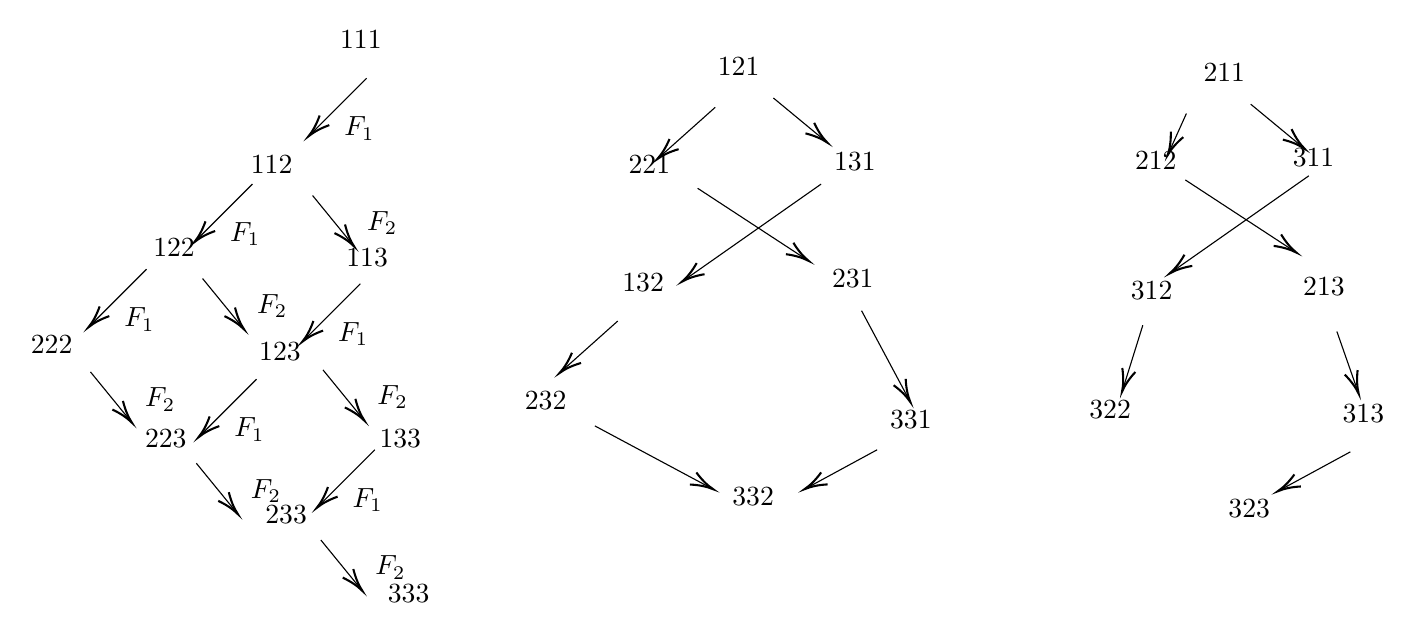
\begin{tikzpicture}[x=0.75pt,y=0.75pt,yscale=-1,xscale=1]
%uncomment if require: \path (0,300); %set diagram left start at 0, and has height of 300

%Straight Lines [id:da42089973349634247] 
\draw    (179,27.5) -- (152.41,54.09) ;
\draw [shift={(151,55.5)}, rotate = 315] [color={rgb, 255:red, 0; green, 0; blue, 0 }  ][line width=0.75]    (10.93,-3.29) .. controls (6.95,-1.4) and (3.31,-0.3) .. (0,0) .. controls (3.31,0.3) and (6.95,1.4) .. (10.93,3.29)   ;
%Straight Lines [id:da3031105581540732] 
\draw    (176,126.5) -- (149.41,153.09) ;
\draw [shift={(148,154.5)}, rotate = 315] [color={rgb, 255:red, 0; green, 0; blue, 0 }  ][line width=0.75]    (10.93,-3.29) .. controls (6.95,-1.4) and (3.31,-0.3) .. (0,0) .. controls (3.31,0.3) and (6.95,1.4) .. (10.93,3.29)   ;
%Straight Lines [id:da803008915658254] 
\draw    (124,78.5) -- (97.41,105.09) ;
\draw [shift={(96,106.5)}, rotate = 315] [color={rgb, 255:red, 0; green, 0; blue, 0 }  ][line width=0.75]    (10.93,-3.29) .. controls (6.95,-1.4) and (3.31,-0.3) .. (0,0) .. controls (3.31,0.3) and (6.95,1.4) .. (10.93,3.29)   ;
%Straight Lines [id:da8767210663804941] 
\draw    (73,119.5) -- (46.41,146.09) ;
\draw [shift={(45,147.5)}, rotate = 315] [color={rgb, 255:red, 0; green, 0; blue, 0 }  ][line width=0.75]    (10.93,-3.29) .. controls (6.95,-1.4) and (3.31,-0.3) .. (0,0) .. controls (3.31,0.3) and (6.95,1.4) .. (10.93,3.29)   ;
%Straight Lines [id:da11711889811973819] 
\draw    (126,172.5) -- (99.41,199.09) ;
\draw [shift={(98,200.5)}, rotate = 315] [color={rgb, 255:red, 0; green, 0; blue, 0 }  ][line width=0.75]    (10.93,-3.29) .. controls (6.95,-1.4) and (3.31,-0.3) .. (0,0) .. controls (3.31,0.3) and (6.95,1.4) .. (10.93,3.29)   ;
%Straight Lines [id:da5343444040412961] 
\draw    (183,206.5) -- (156.41,233.09) ;
\draw [shift={(155,234.5)}, rotate = 315] [color={rgb, 255:red, 0; green, 0; blue, 0 }  ][line width=0.75]    (10.93,-3.29) .. controls (6.95,-1.4) and (3.31,-0.3) .. (0,0) .. controls (3.31,0.3) and (6.95,1.4) .. (10.93,3.29)   ;
%Straight Lines [id:da8170158271849678] 
\draw    (153,84) -- (171.74,106.95) ;
\draw [shift={(173,108.5)}, rotate = 230.77] [color={rgb, 255:red, 0; green, 0; blue, 0 }  ][line width=0.75]    (10.93,-3.29) .. controls (6.95,-1.4) and (3.31,-0.3) .. (0,0) .. controls (3.31,0.3) and (6.95,1.4) .. (10.93,3.29)   ;
%Straight Lines [id:da2307297886745664] 
\draw    (100,124) -- (118.74,146.95) ;
\draw [shift={(120,148.5)}, rotate = 230.77] [color={rgb, 255:red, 0; green, 0; blue, 0 }  ][line width=0.75]    (10.93,-3.29) .. controls (6.95,-1.4) and (3.31,-0.3) .. (0,0) .. controls (3.31,0.3) and (6.95,1.4) .. (10.93,3.29)   ;
%Straight Lines [id:da7984622676548068] 
\draw    (46,169) -- (64.74,191.95) ;
\draw [shift={(66,193.5)}, rotate = 230.77] [color={rgb, 255:red, 0; green, 0; blue, 0 }  ][line width=0.75]    (10.93,-3.29) .. controls (6.95,-1.4) and (3.31,-0.3) .. (0,0) .. controls (3.31,0.3) and (6.95,1.4) .. (10.93,3.29)   ;
%Straight Lines [id:da5520008445276355] 
\draw    (158,168) -- (176.74,190.95) ;
\draw [shift={(178,192.5)}, rotate = 230.77] [color={rgb, 255:red, 0; green, 0; blue, 0 }  ][line width=0.75]    (10.93,-3.29) .. controls (6.95,-1.4) and (3.31,-0.3) .. (0,0) .. controls (3.31,0.3) and (6.95,1.4) .. (10.93,3.29)   ;
%Straight Lines [id:da1625762686635499] 
\draw    (97,213) -- (115.74,235.95) ;
\draw [shift={(117,237.5)}, rotate = 230.77] [color={rgb, 255:red, 0; green, 0; blue, 0 }  ][line width=0.75]    (10.93,-3.29) .. controls (6.95,-1.4) and (3.31,-0.3) .. (0,0) .. controls (3.31,0.3) and (6.95,1.4) .. (10.93,3.29)   ;
%Straight Lines [id:da1026725922353392] 
\draw    (157,250) -- (175.74,272.95) ;
\draw [shift={(177,274.5)}, rotate = 230.77] [color={rgb, 255:red, 0; green, 0; blue, 0 }  ][line width=0.75]    (10.93,-3.29) .. controls (6.95,-1.4) and (3.31,-0.3) .. (0,0) .. controls (3.31,0.3) and (6.95,1.4) .. (10.93,3.29)   ;
%Straight Lines [id:da4681112463331931] 
\draw    (375,37) -- (399.46,57.23) ;
\draw [shift={(401,58.5)}, rotate = 219.59] [color={rgb, 255:red, 0; green, 0; blue, 0 }  ][line width=0.75]    (10.93,-3.29) .. controls (6.95,-1.4) and (3.31,-0.3) .. (0,0) .. controls (3.31,0.3) and (6.95,1.4) .. (10.93,3.29)   ;
%Straight Lines [id:da657993683720376] 
\draw    (347,41.5) -- (320.49,65.17) ;
\draw [shift={(319,66.5)}, rotate = 318.24] [color={rgb, 255:red, 0; green, 0; blue, 0 }  ][line width=0.75]    (10.93,-3.29) .. controls (6.95,-1.4) and (3.31,-0.3) .. (0,0) .. controls (3.31,0.3) and (6.95,1.4) .. (10.93,3.29)   ;
%Straight Lines [id:da23694615966603938] 
\draw    (398,78.5) -- (332.64,124.35) ;
\draw [shift={(331,125.5)}, rotate = 324.95] [color={rgb, 255:red, 0; green, 0; blue, 0 }  ][line width=0.75]    (10.93,-3.29) .. controls (6.95,-1.4) and (3.31,-0.3) .. (0,0) .. controls (3.31,0.3) and (6.95,1.4) .. (10.93,3.29)   ;
%Straight Lines [id:da6217535822776135] 
\draw    (338.5,80.5) -- (390.33,114.41) ;
\draw [shift={(392,115.5)}, rotate = 213.19] [color={rgb, 255:red, 0; green, 0; blue, 0 }  ][line width=0.75]    (10.93,-3.29) .. controls (6.95,-1.4) and (3.31,-0.3) .. (0,0) .. controls (3.31,0.3) and (6.95,1.4) .. (10.93,3.29)   ;
%Straight Lines [id:da6082139480648872] 
\draw    (300,144.5) -- (273.49,168.17) ;
\draw [shift={(272,169.5)}, rotate = 318.24] [color={rgb, 255:red, 0; green, 0; blue, 0 }  ][line width=0.75]    (10.93,-3.29) .. controls (6.95,-1.4) and (3.31,-0.3) .. (0,0) .. controls (3.31,0.3) and (6.95,1.4) .. (10.93,3.29)   ;
%Straight Lines [id:da3195984051533788] 
\draw    (289,195) -- (344.24,224.56) ;
\draw [shift={(346,225.5)}, rotate = 208.15] [color={rgb, 255:red, 0; green, 0; blue, 0 }  ][line width=0.75]    (10.93,-3.29) .. controls (6.95,-1.4) and (3.31,-0.3) .. (0,0) .. controls (3.31,0.3) and (6.95,1.4) .. (10.93,3.29)   ;
%Straight Lines [id:da6108309460864101] 
\draw    (425,206.5) -- (391.76,224.55) ;
\draw [shift={(390,225.5)}, rotate = 331.5] [color={rgb, 255:red, 0; green, 0; blue, 0 }  ][line width=0.75]    (10.93,-3.29) .. controls (6.95,-1.4) and (3.31,-0.3) .. (0,0) .. controls (3.31,0.3) and (6.95,1.4) .. (10.93,3.29)   ;
%Straight Lines [id:da2663257070875219] 
\draw    (417.5,139.5) -- (440.06,181.74) ;
\draw [shift={(441,183.5)}, rotate = 241.89] [color={rgb, 255:red, 0; green, 0; blue, 0 }  ][line width=0.75]    (10.93,-3.29) .. controls (6.95,-1.4) and (3.31,-0.3) .. (0,0) .. controls (3.31,0.3) and (6.95,1.4) .. (10.93,3.29)   ;
%Straight Lines [id:da41104506477492275] 
\draw    (605,40) -- (612.56,46.25) -- (629.46,60.23) ;
\draw [shift={(631,61.5)}, rotate = 219.59] [color={rgb, 255:red, 0; green, 0; blue, 0 }  ][line width=0.75]    (10.93,-3.29) .. controls (6.95,-1.4) and (3.31,-0.3) .. (0,0) .. controls (3.31,0.3) and (6.95,1.4) .. (10.93,3.29)   ;
%Straight Lines [id:da3109726409881449] 
\draw    (574,44.5) -- (565.82,62.68) ;
\draw [shift={(565,64.5)}, rotate = 294.23] [color={rgb, 255:red, 0; green, 0; blue, 0 }  ][line width=0.75]    (10.93,-3.29) .. controls (6.95,-1.4) and (3.31,-0.3) .. (0,0) .. controls (3.31,0.3) and (6.95,1.4) .. (10.93,3.29)   ;
%Straight Lines [id:da4421494524769354] 
\draw    (633,74.5) -- (567.64,120.35) ;
\draw [shift={(566,121.5)}, rotate = 324.95] [color={rgb, 255:red, 0; green, 0; blue, 0 }  ][line width=0.75]    (10.93,-3.29) .. controls (6.95,-1.4) and (3.31,-0.3) .. (0,0) .. controls (3.31,0.3) and (6.95,1.4) .. (10.93,3.29)   ;
%Straight Lines [id:da32714587117225613] 
\draw    (573.5,76.5) -- (625.33,110.41) ;
\draw [shift={(627,111.5)}, rotate = 213.19] [color={rgb, 255:red, 0; green, 0; blue, 0 }  ][line width=0.75]    (10.93,-3.29) .. controls (6.95,-1.4) and (3.31,-0.3) .. (0,0) .. controls (3.31,0.3) and (6.95,1.4) .. (10.93,3.29)   ;
%Straight Lines [id:da203922877186004] 
\draw    (553,146.5) -- (543.6,176.59) ;
\draw [shift={(543,178.5)}, rotate = 287.35] [color={rgb, 255:red, 0; green, 0; blue, 0 }  ][line width=0.75]    (10.93,-3.29) .. controls (6.95,-1.4) and (3.31,-0.3) .. (0,0) .. controls (3.31,0.3) and (6.95,1.4) .. (10.93,3.29)   ;
%Straight Lines [id:da4533498811545599] 
\draw    (646.5,149.5) -- (656.34,177.61) ;
\draw [shift={(657,179.5)}, rotate = 250.71] [color={rgb, 255:red, 0; green, 0; blue, 0 }  ][line width=0.75]    (10.93,-3.29) .. controls (6.95,-1.4) and (3.31,-0.3) .. (0,0) .. controls (3.31,0.3) and (6.95,1.4) .. (10.93,3.29)   ;
%Straight Lines [id:da31860421298697295] 
\draw    (653,207.5) -- (619.76,225.55) ;
\draw [shift={(618,226.5)}, rotate = 331.5] [color={rgb, 255:red, 0; green, 0; blue, 0 }  ][line width=0.75]    (10.93,-3.29) .. controls (6.95,-1.4) and (3.31,-0.3) .. (0,0) .. controls (3.31,0.3) and (6.95,1.4) .. (10.93,3.29)   ;

% Text Node
\draw (165,3.4) node [anchor=north west][inner sep=0.75pt]    {$111$};
% Text Node
\draw (122,63.4) node [anchor=north west][inner sep=0.75pt]    {$112$};
% Text Node
\draw (168,108.4) node [anchor=north west][inner sep=0.75pt]    {$113$};
% Text Node
\draw (126,153.4) node [anchor=north west][inner sep=0.75pt]    {$123$};
% Text Node
\draw (75,103.4) node [anchor=north west][inner sep=0.75pt]    {$122$};
% Text Node
\draw (16,150.4) node [anchor=north west][inner sep=0.75pt]    {$222$};
% Text Node
\draw (71,195.4) node [anchor=north west][inner sep=0.75pt]    {$223$};
% Text Node
\draw (184,195.4) node [anchor=north west][inner sep=0.75pt]    {$133$};
% Text Node
\draw (129,232.4) node [anchor=north west][inner sep=0.75pt]    {$233$};
% Text Node
\draw (188,270.4) node [anchor=north west][inner sep=0.75pt]    {$333$};
% Text Node
\draw (167,44.9) node [anchor=north west][inner sep=0.75pt]    {$F_{1}$};
% Text Node
\draw (164,143.9) node [anchor=north west][inner sep=0.75pt]    {$F_{1}$};
% Text Node
\draw (112,95.9) node [anchor=north west][inner sep=0.75pt]    {$F_{1}$};
% Text Node
\draw (61,136.9) node [anchor=north west][inner sep=0.75pt]    {$F_{1}$};
% Text Node
\draw (114,189.9) node [anchor=north west][inner sep=0.75pt]    {$F_{1}$};
% Text Node
\draw (171,223.9) node [anchor=north west][inner sep=0.75pt]    {$F_{1}$};
% Text Node
\draw (178,104.1) node [anchor=south west] [inner sep=0.75pt]    {$F_{2}$};
% Text Node
\draw (125,144.1) node [anchor=south west] [inner sep=0.75pt]    {$F_{2}$};
% Text Node
\draw (71,189.1) node [anchor=south west] [inner sep=0.75pt]    {$F_{2}$};
% Text Node
\draw (183,188.1) node [anchor=south west] [inner sep=0.75pt]    {$F_{2}$};
% Text Node
\draw (122,233.1) node [anchor=south west] [inner sep=0.75pt]    {$F_{2}$};
% Text Node
\draw (182,270.1) node [anchor=south west] [inner sep=0.75pt]    {$F_{2}$};
% Text Node
\draw (347,16.4) node [anchor=north west][inner sep=0.75pt]    {$121$};
% Text Node
\draw (403,61.9) node [anchor=north west][inner sep=0.75pt]    {$131$};
% Text Node
\draw (304,63.4) node [anchor=north west][inner sep=0.75pt]    {$221$};
% Text Node
\draw (301,120.4) node [anchor=north west][inner sep=0.75pt]    {$132$};
% Text Node
\draw (402,118.4) node [anchor=north west][inner sep=0.75pt]    {$231$};
% Text Node
\draw (254,177.4) node [anchor=north west][inner sep=0.75pt]    {$232$};
% Text Node
\draw (581,19.4) node [anchor=north west][inner sep=0.75pt]    {$211$};
% Text Node
\draw (548,61.4) node [anchor=north west][inner sep=0.75pt]    {$212$};
% Text Node
\draw (624,60.4) node [anchor=north west][inner sep=0.75pt]    {$311$};
% Text Node
\draw (546,124.4) node [anchor=north west][inner sep=0.75pt]    {$312$};
% Text Node
\draw (629,122.4) node [anchor=north west][inner sep=0.75pt]    {$213$};
% Text Node
\draw (526,181.4) node [anchor=north west][inner sep=0.75pt]    {$322$};
% Text Node
\draw (593,229.4) node [anchor=north west][inner sep=0.75pt]    {$323$};
% Text Node
\draw (648,183.4) node [anchor=north west][inner sep=0.75pt]    {$313$};
% Text Node
\draw (354,223.4) node [anchor=north west][inner sep=0.75pt]    {$332$};
% Text Node
\draw (430,186.4) node [anchor=north west][inner sep=0.75pt]    {$331$};


\end{tikzpicture}

    \end{figure}
    So this first one gives us an adjoint representation, the next one also gives us another adjoint. So this last one for $111$ gives us the last 10 elements. The $321$ gives us the last one. From this the representation decomposes as
    $$V^{(3,0)}\oplus(V^{(2,1)})^(\oplus 2)\oplus V^{(0,0)}.$$
    They all have the same weight but are independent one-dimensional weight spaces. Each word on the $111$ diagram has a different weight. How many words have weight $(1,2)$, its $122,212$ and $221$ so the dimesion of that space is $3=\binom{3}{2}=\binom{3}{1}$. 
\end{Ex}

\begin{Qn}
In $(V^{(1,0)})^{\ox n}$, ¿what is the dimension of the weight space $\al=(a,b,c)=(a-c,b-c)$? It's however many words of length $n$ have $a$ $1'$s, $b$ $2'$s and $c$ $3'$s. This is $\binom{n}{a,b,c}=\frac{n!}{a!b!c!}$, which is counted by taking all the words and then dividing by possible rearrangements. This gives us something with the dots in the diagram. 
\end{Qn}

Recall from when we talked about RSK insertion: It is compatible with $\gsl_2$ crystal operations on tableau reading word. In other words this is, if $\un a\xrightarrow{F_i}\un{b}$ then 
\begin{itemize}
    \item The RSK insertion tableau of $\un a,\un b$ matches.
    \item $\rw(\ins(\un a))\xrightarrow{F_i}\rw(\ins(\un b))$.
\end{itemize}

So in conclusion, each connected component (irreducible representation) in $(V^{(1,0)})^{\ox n}$ corresponds to a recording tableau. Let's see how this works: 

\begin{Ex}
    If we take the RSK insertion of the diagram we get \red{diagram}. The bumping sequence is all the same! What that means is that we can take the reading word and apply $F_1$. So all the stuff we did on crystals in 502 is coming back.\par
    If we take the other one for $211$, the RSK insetion is $\young(2,11)$ but the recording tableau is $\young(2,13)$ so we're gonna count how many times an irreducible representation shows up by counting tableau.
\end{Ex}

\section{Day n+1|20241002}

Recall $(V^{(1,0)})^{\ox n}$ is described by words of $1,2,3$ of length $n$ with $F_1,F_2$ bracketing rules.
$E_1,E_2$ also have bracketing rules. Consider the word
$$1223112133212\to)((?))()??()($$
so $E_1$ changes the leftmost unpaired $2$ to a $1$ which leaves us with 
$$1223112133211\to)((?))()??()).$$
The highest weight is the ballot word which when read right to left has more $\#i$'s than $\#i+1$'s.

\begin{Ex}
    We have $(V^{(1,0)})^{\ox 4}$ with dimension $3^4=81$. The highest weight words, or ballot\footnote{Yamanouchi or reverse ballot} words are
    $$1111,1121,1211,1321,2111,2121,2211,3121,3211$$
    corresponding to 
    $$V^{(4,0)},V^{(3,1)},V^{(3,1)},V^{(2,1,1)}=V^{(1,0)},V^{(3,1)},V^{(2,2)},V^{(2,2)},V^{(1,0)},V^{(1,0)}.$$
    So this is 
    $$V^{(4,0)}\oplus (V^{(3,1)})^{\oplus 3}\oplus(V^{(2,2)})^{\oplus 2}\oplus(V^{(1,0)})^{\oplus 3}.$$
\end{Ex}
Recall that $V^{(2,1,1)}=V^{(1,0)}$ because $L_1+L_2+L_3=0$ and we can quotient out by $(1,1,1)$.\par
Let's recall some crystal/Young tableaux facts:
\begin{enumerate}
    \item RSK recording tableau is unchanged via $F_1,F_2$.
    \item Any highest weight word has RSK insertion tableau that looks like 
    $$\young(33,222,1111)$$
    where all $i'$s are in row $i$ from the bottom.
\end{enumerate}
This facts imply that two connected components of $(V^{(1,0)})^{\ox n}$ crystal have different recording tableau as RSK is a bijection.
\begin{Ex}
    We have that 
    $$3121\xrightarrow{RSK}[[3[]]]$$
\end{Ex}

\section{Day n+2| 20241004}

\subsection*{Characters of $\gsl_3$ representations}

The last time we talked about 
$$\chi(V)=\sum_{\al\in\La}\dim(V_\al)x^\al.$$
There's this fact which is the \emph{highest weight theorem} which states:

\begin{Th}
    $V$ is determined by $\chi(V)$.
\end{Th}

The idea of this for $\gsl_3$ is that we had the hexagonal lattice which was generated by a unique highest weight element.\par
So given $\ch(V)$, let $x^\al$ appear in $\ch(V)$ where $\al$ is a highest weight, subtract $\ch(V^\al)$ and iterate.\par
With the notation 
$$x^\al=x_1^{\al_1}x_2^{\al_2}x_3^{\al_3}$$
we ask what is the character of $V^{(a,b)}$?

\begin{Ex}
    We've written $V^{(1,0)}$ as 
    \begin{center}
        FIGURE
    \end{center}
    Summing up the monomials we can see that this is 
    $$\chi(V^{(2,1)})=s_{(2,1)}\bmod x_1x_2x_3.$$
\end{Ex}

\begin{Prop}
The character of $V^{(a,b)}$ is 
$$\chi(V^{(a,b)})=s_{(a,b)}(x_1,x_2,x_3)\bmod x_1x_2x_3.$$
\end{Prop}

This isn't immediately obvious. We have a bunch of words and insert them, but we need to see that every SSYT occurs.

\begin{ptcbp}
    Recall 
    $$s_{(a,b)}(x_1,x_2,x_3)=\sum_{\substack{T\in SSYT(a,b)\\ 1,2,3}}x^T.$$
    We claim that every SSYT T is obtained from a sequence of $F_1,F_2$'s applied to 
    $$\young(222,11111)$$
    We ought to show we can get back to it with $E's$. Let's do this more generally for $\gsl_n$. If $T$ is not highest weight, we will show that we can apply a raising operator.\par
    Let $r$ be the lowest row such that $T$ doesn't have all $r$'s in that row. Say $r=3$ then in 
    $$\young(45,3345,2222,11111)$$
    we take the rightmost element $i$ of row $r$. This means that $i>r$. This is, in this case $i=5$. We may now apply $E_{i-1}$ which is well defined because in row $r$, there's no $i-1$ below it. Here $i-1\geq r$ for all rows below a  $r-1$.
    So bracketing $i,i-1$ there is an upaired $i$ to which we may apply $E_i$.insertion \red{sleep}
\end{ptcbp}

This first Littlewood Richardson rule is concatenate reading words like in $\gsl_2$. The coefficient is 
$$c_{\la\mu}^\nu=\# \text{pairs} (T,S) \text{of shapes }\la,mu(unfinished)$$
The third LR rule is in terms of skew tableau. The LR coefficient is then $\#$ of skew SSYT of shape $\nu/\la$ and content $\mu$ with a ballot reading word. Proving this is harder but it's not so bad when we think of a skew crystal. It's not obvious what's going on. Recall the Hall inner product which gives us 
$$\braket{s_\mu s_\la}{s_\nu}=c_{\la\mu}^\nu=\braket{s_\mu}{s_{\nu/\la}}.$$

\section{Day n+3| 20241007}

\subsection{Representations of $\gsl_n$}

There's no steps of thinking to this. It's the same as $\gsl_3$. Recall $\gsl_n$ corresponds to $n\x n$ matrices which are traceless. The Cartan subalgebra of $\gsl_n$ is 
$$\lie{h}=\set{\text{diagonal matrices }M,\ \tr M=0}.$$
Then elements here are $H=\diag(x_1,\dots,x_n)$ such that $\sum x_i=0$. To define weights, these live in $\lie h^\ast$ and they are joint eigenvalues of $H$ in a representation $V$ of $\gsl_n$. In other words, $\al\in\lie h^\ast$ with $v_\al\in V$ such that 
$$Hv_\al=\al(H)v_\al,\word{for}H\in\lie h.$$

\begin{Ex}
    If $\al\diag(x_1,\dots,x_n)=x_1$ then this is $L_1$. $L_i$ is such that $L_i\diag(\un x)=x_i$.
\end{Ex}

The \term{weight space} is $L_1+\dots+L_n=0$. What are all the weights which are valid for representations? The weight lattice is $\genr{L_1\dots,L_n}$ and all weights lie on the lattice. The proof proceeds the same way, taking block copies of $\gsl_2$.

\subsection{Adjoint representation of $\gsl_n$}

In $\gsl_3$, the adjoint representation had dimension 8.  

\subsection{Crystals for $\gsl_n$}

$(1,0,\dots,0)=L_1$

\begin{Th}
    $(V^{L_1})^{\ox m}=\bigoplus c_\la V^{\la}$
    where $c_\la=\#SYT(\la)$
\end{Th}

The proof is done using crystals and RSK, every connected component corresponds to a unique recording tableau.

\section{Day n+4| 20241009}

\subsection{$\gsl_n$ crystals and Stembridge axioms}

Consider the word 
$$21132342132$$
we claim that the operations $F_1$ and $F_3$ commute in $\gsl_n$. Observe that $F_1$ brackets $(1,2)$ and $F_3$ brackets $(3,4)$. 
We thus get:
\begin{align*}
    &F_1(21132342132)=21232342132\\
    &F_3(21132342132)=21132442132\\
\end{align*} 
and then applying $F_3,F_1$ respectively we get the same word 
$$21232442132.$$
Sometimes $F_1F_3$ is not defined so we actually mean that 
$$F_1F_3(x)=y\To F_3F_1(x)=y$$
even when $y=0$. We have a lot of commuting squares then! We may generalize to 

\begin{Th}
    $F_i,F_j$ commute when $|i-j|>1$. 
\end{Th}

This characterizes the crystal graphs but not completely, that's where the Stembridge axioms come into play. 

\begin{Th}
    In an $\gsl_n$ crystal, for $F_1(w),F_2(w)$ either:
    \begin{enumerate}
        \item $\exists z (z=F_1F_2(w)=F_2F_1(w))$, or
        \item $\exists u,v,s,t,z$ such that the crystal is just like the adjoint representation. This means that 
        $$F_2F_1F_1F_2=F_1F_2F_2F_1.$$
    \end{enumerate}
\end{Th}

¿Why can't we have more complicated words than that? The proof for this will be very combinatorial and we will analyze a lot of words.

\begin{ptcbp}
    Let $a$ be the rightmost unpaired $1$ in $w$ for $(1,2)$. Then call $b$ the rightmost unpaired $2$ in $w$ for $(2,3)$.
    \begin{itemize}
        \item In the first case, we assume that removing $b$ does not unbracket a $1$. Take for example\red{sleep}
        \item In the next case $F_1F_1F_2$
        \item The third case is basically removing $b=2$ unpairs $c=1$, where $b$ is left of $a$ and there exists and unpaired $3$ to the left of $a$. This is 
        $$-2-1-(3)-1-$$
        so applying $F_1$ gets us $-2132-$ and $F_2$ leaves us with $-3131-$. This both meet up after applying $F_2$ and $F_1$ respectively.
        \item Finally it could be like before but there's no unpaired $3$ left of $a$. Here we get another figure 8 diagram. For this case we get 
    \end{itemize}
    

\end{ptcbp}

This all comes from Stembridge's 2004 paper. 

\section{Day n+5|20241011}

We were talking about how the figure 8 and sqaure characterizes stuff. We will now characterize crystals as graphs. 

\subsection{Crystals of type $A$}

\begin{Def}
A type $A$ \term{Kashiwara} crystal of finite type is
\begin{itemize}
    \item $B$ a crystal base (weight spaces' generators are bases), nonempty set.
    \item Two arrow maps $e_i,f_i\: B\to B\cupdot \set{emptyset}$ for $i\in\bonj{n-1}$.
    \item Two length maps $\eps_i,\vf_i\: B\to\bZ$ which correspond to the number of times you can apply $e_i$ and $f_i$.
    \item And a weight function to thw lattice $\wt\: B\to\La$ where $\La\bZ\genr{L_1,\dots,L_n}$ and $\sum L_i=0$. Elements here are $\un a/\un 1$, i.e. modded by translations.
\end{itemize}
They must satisfy the properties
\begin{enumerate}
    \item If $x,y\in B$, then 
    $$e_i(X)=y\iff x=f_i(y)$$
    and in this case
    $$\wt(y)=\wt(x)+\al_i$$
    where $\al_i=(0,0,\dots,1,-1,0,\dots,0)$ with $1$ in position $i$ and $-1$ in the next one.\par
    And also 
    $$\vf_i(y)=\vf_i(x)+1.$$
    \item For all $i,x_i$ 
    $$\vf_i(x)-\eps_i(x)=\wt(x)_i-\wt(x)_{i+1}.$$
    To state this for general crystals we need an inner product.
\end{enumerate}
\end{Def}

\begin{Ej}
Analyze how tableaux crystals fit into this picture.
\end{Ej}

\begin{Ex}
    In $n=2$, we had $\gsl_2$ but now we can make an infinite chain. Let us take our basis 
    $$B=\set{v_0,v_{-2},v_{-4},\dots}$$
    where the $f$ arrow 
\end{Ex}

\section{Day n+6|20241014}

Recall the Stembridge axioms, $(B,e_i,f_i,\eps_i,\vf_i,\wt)$. 

\begin{enumerate}
    \item seminormality
    \item length axioms
    \item diamond shape
    \item figure 8
\end{enumerate}

So let us finish the proof 

\begin{Th}
    Connecteed Stembridge crystals are crystals whose graph is connected. They have a unique highest weight element (unique maximal, all $e_i$'s send it to zero).
\end{Th}

\begin{ptcbp}
    Let $x$ be a highest weight element, assume for contradiction it's not unique. Let us define 
    $$S=\set{z_i\:\ \exists f_{i_1},\dots,f_{i_k},\ f_{i_1}\circ\dots\circ f_{i_k}x=z}=\set{\text{pts. below }x}.$$
    There could be some other stuff not below $x$, outside $S$. Let us take $z\in S$ be maximal (in the crystal) such that $z$ is covered by some $y$ not in $S$. This is the highest $z$ which has something from the outside pointing to it.\par
    We have that $z\neq x$ as $x$ is maximal (highest weight) by assumption (otherwise $y\to x$, contradiction). Let $z'\in S$, $f_i(z')=z$ for some $i$.\par
    If $S2'$ applies, then there's a $w$ 
    $$w\xrightarrow{f_j}z',\quad w\xrightarrow{f_i}y,$$
    because $z$ was maximal, $w\in S$.\par
    \begin{enumerate}
        \item $S1$ implies that if $f_i(x)=y$
        \item \red{sleep}
    \end{enumerate}
\end{ptcbp}

\begin{Th}
    If two connected Stembridge crystals $C,C'$ have highest weight elements $x,x'$ and weight $\wt(x)=\wt(x')$ then $C\isom C'$. This means that we get the same graph, weight, $\vf_i,\eps_i$ values.
\end{Th}

This theorem is proved in Shilling and Bald's book. The idea starts with the weight function, axiom $K2$ relates weight with $\eps_i,\vf_i$. Then by induction each successive row starting from the top is determined. (Row means how many $f$'s you have to apply to get there. Can't have non-graded posets) This is uniquely determined via $S1,S2$ and $S3$.\par
We can now connect this with Lie algebras.

\begin{Cor}
    Every Stembridge crystal is isomorphic to a crystal of tableaux.
\end{Cor}

\begin{ptcbp}
    Tableaux crystals satisfy $K_1,K_2$ and $S0$ through $S3'$. And every highest weight appears as the highest weight of some tableau crystal. So by the previous theorem, we are done.
\end{ptcbp}

\begin{Rmk}
    It is hard to find local axioms to globally determine the structure of the crystal. Recall that we know that the character of a Stembridge crystal $\chi(V^\la)=s_\la$ (irreducible representation of $\gsl_n$), then 
    $$\chi(C)=\sum_{b\in C} x^{\wt(b)}$$
    sum is over dots of the crystal. So 
    $$\chi(\text{tableau crystal }C^\la)=s_\la.$$
\end{Rmk}

\begin{Cor}
    Say we have a symmetric function $f=\sum c_\la s_\la$. If we want to show $c_\la\in\bZ_{\geq 0}$, then if the symmetric function is of the form $f=\sum x^P$, then the method is to try to define raising and lowering operators such that Stembridge's axioms are satisfied. 
\end{Cor}

This method has been done a few times now. Stanley symmetric functions and ordered symmetric functions are some of the examples where this can be used.

\subsection{Beyond type $A$: General Lie algebras and Root systems}

Recall $\lie g$ is a $\bC$-vector space with a Lie bracket. Any Lie algebra has a system of roots. 

\begin{Def}
The roots of $\lie g$ are weights of the adjoint representation acting on itself via the Lie bracket.\par
The Cartan subalgebra $\lie h$ is the maximal Abelian Lie subalgebra.
\end{Def}

\begin{Def}
We say $\lie g$ is semisimple if its roots span $\lie h^\ast$.
\end{Def}

\begin{Ex}
    Recall $\ggl_n$ is the whole set of $n\x n$ matrices. The roots of $\ggl_n$ are $L_i\diag(\un x)=x_i$, $L_i-L_j$ for $i\neq j$. This is the same as $\gsl_n$, but the weight space is $\genr{L_1,\dots,L_n}$ which is not $\genr{L_1,\dots,L_n}/\sum L_i=0$ which is $\gsl_n$'s weight space.
\end{Ex}

The goal is to classify semisimple Lie algebras by classifying sets of roots. We will use certain facts about Lie algebras:

\begin{Prop}
    For a semisimple Lie algebra $\lie g$ the following hold:
    \begin{enumerate}
        \item $\lie g=\lie h\oplus\bigoplus_{\al\in R}\lie g_\al$ where $\lie g_\al$ is 1 dimensional. Say for example $\lie g_{L_1-L_2}=\genr{E_{12}}$.
        \item Little $\gsl_2$'s for each root. $\lie g_\al\oplus\lie g_{-\al}\oplus\bonj{\lie g_\al,\lie g_{-\al}}\hookto\lie g$. In our case this correspond to $E,F$ and $H$.
    \end{enumerate}
\end{Prop}

\section{Day n+7|20241016}

\subsection{General Lie algebra representation theoru and root systems}

Recall that the adjoint representation of a Lie algebra decomposes as 
$$\lie g=\lie h\oplus\bigoplus_{\al\in R}\lie g_\al$$
where $R$ is a set of roots which are non-zero weights of $\Ad(\lie g)$. We have the properties
\begin{itemize}
    \item Each $\lie g_\al$ is 1 dimensional.
    \item For $\al\in R$ we also have $-\al\in R$.
    \item We will have little $\gsl_2$:
    $$(\gsl_2)_\al=\lie g_\al\oplus\lie g_{-\al}\oplus\bonj{\lie g_\al,\lie g_{-\al}}.$$
    \item In $\lie h$ choose a hyperplane, positive roots and simple roots (roots which are not a positive sum of other positive roots.)
    \item Positive simple roots are in correspondence with raising operators $E_\al,\ \al\in R^+$.
\end{itemize}

From this highest weight is such that it is killed by all the raising operator.

\begin{Def}
    A vector $v\in V$ is of \term{highest weight} if $E_\al v=0$ for all $\al\in R^+$.
\end{Def}

\begin{Prop}
    Irreducible representations of any semisimple $\g$ have a unique highest weight vector, one for each highest weight $V^\bt$ is the irreducible representation with highest weight 
\end{Prop}

\section{Day n+8|20241018}

\subsection{Root systems}

Recall a root system in an inner product space is a finite set $R$ with 

\begin{enumerate}
    \item $r_\al(\bt)\in R$ for all $\al,\bt$ where
    $$r_\al(\bt)=\bt-\frac{2\braket{\bt}{al}}{\braket{\al}{\al}}\al.$$
    \item The coefficient $\frac{2\braket{\bt}{al}}{\braket{\al}{\al}}\al$ is an integer.
    \item If $\bt=\la\al$ then $\la=\pm1$.
\end{enumerate}

\begin{Ex}
    All the root systems that fit in two dimensions are
    \begin{enumerate}
        \item For $\gsl_n$: $R=\set{L_i-L_j}$ and positive roots $R^+=\set{L_i-L_j\: i<j}$ and the simple roots $R^+_0=\set{L_i-L_{i+1}\: i\in\bonj{n-1}}$.
        \item For $\gsl_3$, we have $L_1-L_2$ and $L_2-L_3$.
    \end{enumerate}
\end{Ex}

\begin{Ej}
    Draw the root system of $\gsl_4$.
\end{Ej}

\begin{Ex}
    For type \red{sleep}
\end{Ex}

\section{Day n+9|20241021}

\subsection{CLassifying root systems}

Last time we connected root systems with Dynkin diagrams. Let's prove some lemmas:

\begin{Lem}
    In a root system $R$, if $\al,\bt$ are two roots, their configuration (if $|\al|=1$) is one of the following:
    \red{Add figure}
\end{Lem}

\begin{ptcbp}
    By definition of root system, we have 
    $$\frac{2\braket{\bt}{\al}}{\braket{\bt}{\bt}}=\frac{2|\al||\bt|\cos(\te)}{|\bt|^2}=\frac{2\cos(\te)|\al|}{\bt}\in\bZ$$
    but also 
    $$\frac{2\braket{\al}{\bt}}{\braket{\al}{\al}}=\frac{2\cos(\te)|\bt|}{|\al|}\in\bZ.$$
    If we normalize by $|\al|$ then in particular we have 
    $$2|\bt|\cos(\te)\.\frac{2\cos(\te)}{|\bt|}\in\bZ$$
    there's not that many values of $\te$ such that $4\cos^2(\te)\in\bZ$. As $\cos^2(\te)\leq 1$, our expression is smaller than 4. Our possibilities are
    $$\cos^2(\te)=0,\frac{1}{4},\frac{2}{4},\frac{3}{4},1\To\cos(\te)=0,\pm\half,\pm\frac{1}{\sqrt{2}},\pm\frac{\sqrt{3}}{2},\pm 1.$$
    This gives us the angles
    $$0,\pi,\pi/6,5\pi/6,\pi/4,3\pi/4,\pi/3,2\pi/3,\pi/2$$
    and for the lengths, take for example $\te=\pi/6$, then 
    $$\frac{\sqrt{3}}{|\bt|},\quad\sqrt{3}|\bt|\in\bZ\To|\bt|=\sqrt{3}.$$
\end{ptcbp}

It really limits the possibilities, so there's only so many finite semisimple Lie algebras. An important corollary of this is:

\begin{Cor}
    If $\al,\bt$ are simple roots, then their angle $\te$ is one of 
    $$\pi/2,2\pi/3,3\pi/4,5\pi/6,$$
    which means that only obtuse angles occur, or in other words, simple roots can't form acute angles. 
\end{Cor}

\begin{ptcbp}
    Recall that simple roots are positive roots which are not sums of other positive roots, where positive roots were positive relative to a hyperplane.\par
    \begin{enumerate}
        \item Suppose $\te=\pi/3$ for example, then if $\al,\bt$ are length 1, we may reflect $\al$ across $\bt$ to get another root. If $\al'$ was such a root, then $\al+\al'=\bt$. If $\al'\in R^+$, then this is a contradiction as $\bt$ is simple.\par
        Otherwise, the reflection of $\bt$ across $\al$ is still in $R^+$ so that $\bt+\bt'=\al$.  
    \end{enumerate}
    Similar cases involve discarding cases like this.
\end{ptcbp}

The point is that simple roots are the roots close to the hyperplane instead of the ones pointing up.

\begin{Def}
    The \term{Dynkin diagram} of a root system is a multigraph whose vertices are the roots and the edges are as follows:
    \begin{itemize}
        \item There's no edge between $\al,\bt$ if $\al\perp\bt$.
        \item There's an edge between them if $\braket{\al}{\bt}=-\half$.
        \item There's two edges if $\braket{\al}{\bt}=-1$ as $\te=\frac{3\pi}{4}$.
        \item Three edges if the angle is $\frac{5\pi}{6}$, in this case $\braket{\al}{\bt}=-\frac{3}{2}$.
    \end{itemize}
\end{Def}

\begin{Qn}
    ¿Why can't simple roots be $\pi$ apart?
\end{Qn}

This is a subtlety, as both roots are $\al,-\al$. They can't be both positive as the hyperplane cuts both of them. We wiggle it a bit and get that they can't be both positive.\par
We will classify Dynkin diagrams. 

\begin{Ex}
    One of the type $B_2$ systems was 

    \begin{center}
        

\tikzset{every picture/.style={line width=0.75pt}} %set default line width to 0.75pt        

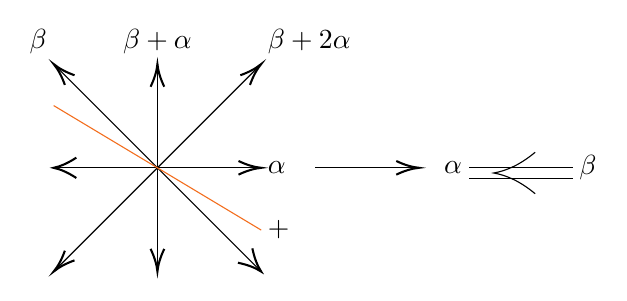
\begin{tikzpicture}[x=0.75pt,y=0.75pt,yscale=-1,xscale=1]
%uncomment if require: \path (0,300); %set diagram left start at 0, and has height of 300

%Straight Lines [id:da3322334110784373] 
\draw    (74,32) -- (74,128) ;
\draw [shift={(74,130)}, rotate = 270] [color={rgb, 255:red, 0; green, 0; blue, 0 }  ][line width=0.75]    (10.93,-3.29) .. controls (6.95,-1.4) and (3.31,-0.3) .. (0,0) .. controls (3.31,0.3) and (6.95,1.4) .. (10.93,3.29)   ;
\draw [shift={(74,30)}, rotate = 90] [color={rgb, 255:red, 0; green, 0; blue, 0 }  ][line width=0.75]    (10.93,-3.29) .. controls (6.95,-1.4) and (3.31,-0.3) .. (0,0) .. controls (3.31,0.3) and (6.95,1.4) .. (10.93,3.29)   ;
%Straight Lines [id:da8255689861417552] 
\draw    (122,80) -- (26,80) ;
\draw [shift={(24,80)}, rotate = 360] [color={rgb, 255:red, 0; green, 0; blue, 0 }  ][line width=0.75]    (10.93,-4.9) .. controls (6.95,-2.3) and (3.31,-0.67) .. (0,0) .. controls (3.31,0.67) and (6.95,2.3) .. (10.93,4.9)   ;
\draw [shift={(124,80)}, rotate = 180] [color={rgb, 255:red, 0; green, 0; blue, 0 }  ][line width=0.75]    (10.93,-3.29) .. controls (6.95,-1.4) and (3.31,-0.3) .. (0,0) .. controls (3.31,0.3) and (6.95,1.4) .. (10.93,3.29)   ;
%Straight Lines [id:da9179385701900346] 
\draw    (25.41,31.41) -- (122.59,128.59) ;
\draw [shift={(124,130)}, rotate = 225] [color={rgb, 255:red, 0; green, 0; blue, 0 }  ][line width=0.75]    (10.93,-4.9) .. controls (6.95,-2.3) and (3.31,-0.67) .. (0,0) .. controls (3.31,0.67) and (6.95,2.3) .. (10.93,4.9)   ;
\draw [shift={(24,30)}, rotate = 45] [color={rgb, 255:red, 0; green, 0; blue, 0 }  ][line width=0.75]    (10.93,-3.29) .. controls (6.95,-1.4) and (3.31,-0.3) .. (0,0) .. controls (3.31,0.3) and (6.95,1.4) .. (10.93,3.29)   ;
%Straight Lines [id:da8483315356097146] 
\draw    (122.59,31.41) -- (25.41,128.59) ;
\draw [shift={(24,130)}, rotate = 315] [color={rgb, 255:red, 0; green, 0; blue, 0 }  ][line width=0.75]    (10.93,-3.29) .. controls (6.95,-1.4) and (3.31,-0.3) .. (0,0) .. controls (3.31,0.3) and (6.95,1.4) .. (10.93,3.29)   ;
\draw [shift={(124,30)}, rotate = 135] [color={rgb, 255:red, 0; green, 0; blue, 0 }  ][line width=0.75]    (10.93,-3.29) .. controls (6.95,-1.4) and (3.31,-0.3) .. (0,0) .. controls (3.31,0.3) and (6.95,1.4) .. (10.93,3.29)   ;
%Straight Lines [id:da788618555786849] 
\draw [color={rgb, 255:red, 243; green, 112; blue, 33 }  ,draw opacity=1 ]   (24,50) -- (124,110) ;
%Straight Lines [id:da45211215260330606] 
\draw    (274,80) -- (224,80) ;
%Straight Lines [id:da18662234610132444] 
\draw    (274,85) -- (224,85) ;
\draw   (256,92.5) .. controls (249.33,86.94) and (242.67,83.61) .. (236,82.5) .. controls (242.67,81.39) and (249.33,78.06) .. (256,72.5) ;
%Straight Lines [id:da5348239421294798] 
\draw    (198,80) -- (150,80) ;
\draw [shift={(200,80)}, rotate = 180] [color={rgb, 255:red, 0; green, 0; blue, 0 }  ][line width=0.75]    (10.93,-3.29) .. controls (6.95,-1.4) and (3.31,-0.3) .. (0,0) .. controls (3.31,0.3) and (6.95,1.4) .. (10.93,3.29)   ;

% Text Node
\draw (22,26.6) node [anchor=south east] [inner sep=0.75pt]    {$\beta $};
% Text Node
\draw (126,80) node [anchor=west] [inner sep=0.75pt]    {$\alpha $};
% Text Node
\draw (126,110) node [anchor=west] [inner sep=0.75pt]    {$+$};
% Text Node
\draw (222,80) node [anchor=east] [inner sep=0.75pt]    {$\alpha $};
% Text Node
\draw (276,80) node [anchor=west] [inner sep=0.75pt]    {$\beta $};
% Text Node
\draw (74,26.6) node [anchor=south] [inner sep=0.75pt]    {$\beta +\alpha $};
% Text Node
\draw (126,26.6) node [anchor=south west] [inner sep=0.75pt]    {$\beta +2\alpha $};


\end{tikzpicture}

    \end{center}
\end{Ex}

\begin{Ex}
    Another was $G_2$, \red{add figure}
\end{Ex}

We will get the graph structure by using undirected Dynkin diagrams. These correspond to normalized root systems.

\begin{Def}
    An \term{admissible diagram} is a graph with $n$ vertices representing $n$ independent unit vectors $e_1,\dots,e_n$ with angles $\te_{ij}$ being in 
    $$\Set{\frac{\pi}{2},\frac{2\pi}{3},\frac{3\pi}{4},\frac{5\pi}{6}}.$$
    In each of these cases we draw no, one, two and three edges respectively but without the arrows.
\end{Def}

After finding the graph shapes, we will add the orientation again. Further we will show that admissible diagrams are trees, vertices have degree 3 and much more.

\section{Day n+10|20241023}

\subsection{Admissible diagrams}

Maria has been looking up to this moment the whole morning. Recall that the setup is that we have $n$ unit vectors which are independent in $\bR^N$:
\begin{itemize}
    \item We have $e_1,\dots,e_n$ independent vectors.
    \item The length of the angle classifies the edges.
\end{itemize}

\section{Day n+12|20241028}

\subsection{Weyl Groups}

We went up to Lie groups, representations of Lie algebras and now we are going back to finite groups once again.\par
Recall that given a root system $R$, for $\al,\bt\in R$, the reflection of $\bt$ through $H_\al$ is 
$$r_\al(\bt)=\bt-\frac{2\braket{\bt}{\al}}{\braket{\al}{\al}}\al.$$
\begin{Def}
    A simple reflection $s_\al$ is $r_\al$ when $\al$ is a simple root. The Weyl group of $R$ is the group of reflections generated by $s_\al$. It is a subgroup of all reflections in $n$-space.
\end{Def}

In particular this is a subgroup of $\rGL_n$. For a root system, this is a finite group. We can also think of them as acting on the roots. 

\begin{Lem}
    Weyl groups are finete and are generated by simple reflections.
\end{Lem}

$W$ acts on the root system by permutations, so $W\subseteq\Sym(R)$ because the induced permutation on the roots has to determine the transformation.\par
In general, we should show that if $\bt=\al+\al'$ then we can express $s_\bt$ in terms of $s_\al,s_{\al'}$.

\begin{Prop}
    Let $s_i,s_j$ be simple reflections (generators in a Weyl group $W$). Then 
    \begin{itemize}
        \item $s_i^2=s_j^2=1$, and
        \item $\exists m_{ij}(s_is_j)^{m_{ij}}=1$ where $m_{ij}\in\set{2,3,4,6}$ is minimal. In other words, it's the order.
    \end{itemize}
\end{Prop}

Observe that it's not necessary that $m_{ij}=2$ always as $s_i,s_j$ may not necessarilly commute.

\begin{ptcbp}
    For the first item, observe that $s_i,s_j$ are involutions. So immediately we get the result. Now let's analyze cases. Simple reflections correspond to nodes of the Dynkin diagram. Take roots $\al_i,\al_j$:
    \begin{itemize}
        \item If there's no edge between them, then they are orthogonal. Then $s_is_j$ is a rotation by $\pi$. Thus $s_i,s_j$ commute and $m_{ij}=2$.
        \item If there's one edge, then the angle between $\al_i,\al_j$ is $2\pi/3$. Hyperplanes between the roots differ by $\pi/3$. We can simplify by considering an $\gsl_3$ $L$ diagram. We get 
        $$s_1=(23),\quad s_2=(13)\To s_1s_2s_1=s_2s_1s_2$$
        which is the braid relation. This simplifies to $(s_1s_2)^3=1$.
        \item The third case corresponds to $2$ edges and a $3\pi/4$ angle. This gives us $m_{ij}=4$.
        \item  Finally with $6$ edges and a $5\pi/6$ angle we get $m_{ij}=6$.
    \end{itemize}
\end{ptcbp}

\begin{Th}
    The Weyl group is actually generated by simple reflections modulo the previous relations.
    $$W=\gen(s_i\:\ s_i^2=1,\ (s_is_j)^{m_{ij}}=1).$$
\end{Th}

Weyl groups sit inside a more general class of groups.

\begin{Def}
    A \term{Coxeter group} is the free group generated by $(s_i)_{i\in I}$ such that 
    \begin{itemize}
        \item $s_i^2=1$, and
        \item $(s_is_j)^{m_{ij}}=1$ for $m_{ij}\in\bZ_{\geq 0}$.
    \end{itemize}
\end{Def}

\begin{Ex}
    In type $A$, our Dynkin diagram looks like a line. Assume it's $\al_1\dots\al_5$. Vertices connected by an edge have a braid relation. In this case $W$ is generated by $s_i$'s such that 
    $$s_i^2=1,\ s_is_{i+1}s_i=s_{i+1}s_is_{i+1},\ s_is_j=s_js_i,\ |i-j|\geq 2.$$
    Observe that we have $s_i=(i\ i+1)$ and 
    $$s_is_j=(i\ i+1)(j\ j+1)=s_js_i$$
    when $|i-j|>2$. On a simpler note observe that 
    $$s_1s_2s_1=s_2s_1s_2$$
    because 
    $$(12)(23)(12)=(13)=(23)(12)(23)=321.$$
    This happens in general for any $i$ so that we have the desired braid relation.\par
    It is also possible to show that there's $(n+1)!$ elements by noticing that how $W$ acts on $L_1,\dots,L_n$ determines a permutation, so $|W|\leq (n+1)!$.
 \end{Ex}

 For type $B$, let's go a little smaller. Type $B$ and $C$ have the same Dynkin diagram.

 \begin{Ex}
    In this case let's label the edge between $s_0,s_1$ as the double edge. Between $s_1,s_2$ we have an ordinary braid relation and $s_0$ commutes with $s_2$. But we have the relation 
    $$s_0s_1s_0s_1=s_1s_0s_1s_0.$$
    The model of this group is the hyperoctahedral group, or signed permutations group. Call $s_1=(12),s_2=(23)$, but the element $s_0$ \emph{flips} the sign of the first letter. In list notation
    $$s_0\:\quad -21-3\mapsto 21-3.$$
 \end{Ex}

 \begin{Def}
    A \term{signed permutation} of $[n]$ is a permutation in list notation along with a $+$ or $-$ sign on each letter.
 \end{Def}

 \begin{Ex}
    $5-143-3$ is a signed permutation, here $w\in S_{\bonj{\pm n}}$ such that $w(-i)=-w(i)$ for all $i$.
 \end{Ex}

 Observe that $W_{B_{n}}$ is a subgroup as 
 $$w\sg(-i)=w(-\sg(i))=-w\sg(i).$$

 So in more generality 
 $$s_1=(12)(3)(-3)(-1-2),s_2=(23)(1)(-1)(-2-3).$$
The longer relation holds in this following example:
$$1234\mapsto -1234\mapsto 2-134\mapsto -2-134\mapsto -1-234$$
where this is $s_0s_1s_0s_1$ and the relation also holds. It's also possible to see in cycle notation that we get a 4-cycle.

\section{Day n+13|20241030}

Recall that the Weyl group is the symmetry group of a root system.\par
The type $D_n$ looks like a $Y$, recall that if $s_i,s_j$:
\begin{itemize}
    \item share no edge, we have the relation $s_is_j=s_js_i$, and
    \item if they share an edge we have $s_is_js_i=s_js_is_j$.
\end{itemize}
These are the only relations that we need for $D_n$'s Weyl group. We have that $W_{D_n}\subseteq W_{B_n}$ which was the octahedral group, the group of signed permutations.
\begin{itemize}
    \item $s_i$ will correspond to switching $i$ with $i+1$, and
    \item $s_0$ negates and swaps \emph{the first two entries}. 
\end{itemize}
Observe that
$$1234\xrightarrow{s_0}6534\xrightarrow{s_2}5634\xrightarrow{s_0}2134$$
where as on the other direction 
$$1234\xrightarrow{s_2}1324\xrightarrow{s_0}7524\xrightarrow{s_2}7254$$
\begin{Ej}
    Check
\end{Ej}

\begin{Lem}
    The size of $W_{D_n}$ is $n!2^{n-1}$.
\end{Lem}

This amount is calculated via $n!\sum_{i=1}^{\floor{n/2}}\binom{n}{2i}$.

\begin{Lem}
    $|W_{B_n}|=n!2^n$.
\end{Lem}
Now instead we choose a sign without restrictions, there's 2 ways per entry and there's $n$ entries. This means that $W_{D_n}\rt W_{B_n}$ so it's a normal subgroup and there's possibilities of taking semidirect products and other stuff.

\begin{Def}
    The Weyl group can be defined abstractly as 
    $$\quot{N_G(T)}{T}$$
    where $G$ is a Lie group and $T$ is the torus, the maximal abelian subgroup.
\end{Def}

\begin{Ex}
    For $\rSL_n$, $T$ is the set of diagonal matrices of determinant 1. Then the normalizer, $N_G(T)$ is the permutation matrices times a diagonal matrix. Finall $N_G(T)/T$ is the set of permutation matrices.
\end{Ex}

\begin{Lem}
    The action of $W$ fixes the set of weights of any representation of $\g$.
\end{Lem}

\begin{ptcbp}
    $s_i$ reflects about the hyperplane orthogonal to $\al_i$. The $\gsl_2$ string in $\al_i$ direction is symmetric. That means $s_i(\bt)$ is a weight of $V$ if $\bt$ is a weight.
\end{ptcbp}

Therefore the action of $S_n$ on $A_{n-1}$ is:

\begin{itemize}
    \item Pair $i+1$'s and $i$'s.
    \item The remaining unpaired $i^a(i+1)^b$ are replaced by $i^b(i+1)^a$.
\end{itemize}

The word 
$$iii+1ii+1iii+1\to iii()()ii+1$$

On Friday we will talk about evacuation and on Monday we will talk about Springer theory.\par

There's a vertical symmetry exhibited by type $A$ crystals. Is there a natural involution that gives vertical symmetry of the type $A$ crystals where we swap $F_i$ with $E_{n-i}$? It turns out that taking the action almost does what we want.\par
If $w_0$ is the word $n(n-1)(n-2)\dots321$ so one minimal way of writing it is 
$$\dots(s_1s_2s_3)(s_1s_2)(s_1)$$
This is not the answer, the actual answer is the Schützenberger involution.

\section{Day n+14|20241101}

\subsection{Evacuation}

To evacuate a tableau $T$ we:
\begin{itemize}
    \item Rotate it 180 degrees.
    \item Change all $i$ to $n+1-i$.
    \item Finally JDT rectify.
\end{itemize}

\begin{Ex}
    Evacuate 
    $$\young(3,234,1123)\to\young(4,233,1224)$$
\end{Ex}

Alternatively
\begin{itemize}
    \item Remove bottom left corner $i$,
    \item Rectify,
    \item Fill evacuated outer square with $n+1-i$ and curly decorate it.
    \item Repeated on non-curly until all are curly.
\end{itemize}

Call $\eta$ our first evacuation. Then

\begin{Prop}
\end{Prop}
$\eta$ gives a vertical symmetry of type $A_{n-1}$ crystals under $F_i\leftrightarrow E_{n+1-i}$.

\chapter{Springer Theory}
\section{Day n+15|20241104}
\subsection{Even less details}

There's going to be EVEN LESS DETAIL, look at Maria.com at the end of the webpage for more references to this.\par
The \term{Springer correspondence} is between 
$$\set{\text{irr. reps. of }W_R}\leftrightarrow\set{\text{Nilp. conj. classes in }\gg}.$$
Where nilpotent conjugacy classes come with a representation of the associateed group $A_G$. In type $A$ isn't needed. Depending on opinions, the Springer correspondence is incomplete. However in type $A$ is a bijection. So to obtain information on the Weyl group, we look at the Lie algebra.\par
Not only it's a bijection, it's an \emph{explicit} bijection. This is constructed via the Springer resolution, coming from the geometry of the flag variety.

\begin{Def}
    A \term{flag} is a chain 
    $$V_\8\: 0\subseteq V_1\subseteq V_2\subseteq\dots\subseteq V_n=\bC^n$$ 
    where $\dim V_i=i$.
\end{Def}

\begin{Ex}
    If $e_i$ is the standard basis vector of $\bC^n$, then 
    $$0\subseteq\gen{e_1}\subseteq\gen(e_1,e_2)\subseteq\dots\subseteq\bC^n$$
    is the standard flag.
\end{Ex}

Out of flags we would like to construct manifolds or algebraic varieties. In particular consider $\rGL_n$ acting on flags, $\Fl_n$. The action is 
$$\g\. V_\8\: 0\subseteq gV_1\subseteq gV_2\subseteq\dots\subseteq gV_n.$$

\begin{Ex}
    For $n=2$, consider the standard flag and $g=\twobytwo{0}{1}{1}{0}$. The the standard flag becomes 
    $$0\subseteq\gen(e_2)\subseteq\bC^2.$$
\end{Ex}

\begin{Lem}
    The action of $\rGL_n$ on $\Fl_n$ is transitive.
\end{Lem}

\begin{ptcbp}
    It suffices to show this with the standard flag $E_\8$. Choose the right $g$, given $W_\8$, we can take $g$ as the matrix whose columns are the $(w_i)$'s.
\end{ptcbp}

\begin{Ex}
    The stabilizer of $E_\8$ counts the amount of overcounting. This is 
    $$\Stab(E_\8)=\set{g\:\ g\.E_\8=E_\8}.$$
    Inductively we can show that this stabilizer is the set of upper triangular matrices which are invertible. In conclusion 
    $$\Stab E_\8=B_n.$$
\end{Ex}

\begin{Th}
    $\Fl_n=\rGL_n/B_n.$
\end{Th}

\begin{ptcbp}
    Flags represent cosets 
    $$\set{gB_n\:\ gE_\8=V_\8}.$$
\end{ptcbp}

From this correspondence we inherit the manifold structure of $\rGL_n$. Recall that $\rGL_n$ is a Lie group so the quotient inherits the manifold structure.\par
From this we will now call the flag as the flag variety or manifold. We can embed the flag into projective space via Plücker relations. 

\begin{Ex}
    In different types we have:
    \begin{enumerate}
\item In type $A$, the flag is equivalent to $\rSL_n/B^{\rSL}_n$. 
\item For type $B$, the flag is $\rSO_{2n+1}$ modded by its corresponding Borel subgroup.
    \end{enumerate}
\end{Ex}

Recall that the Borel subgroup is the maximal, closed, connected, solvable subgroup. 

\begin{Rmk}
    Recall that solvable groups are those whose successive commutator subgroups eventually trivialize: $B,B_1=\bonj{B,B}$, $B_2=\bonj{B_1,B_1}$ and so on. 
\end{Rmk}

Let's check it in dimensoin $2$:

\begin{Ex}
    Observe that 
    $$\twobytwo{a}{b}{0}{c}\twobytwo{x}{y}{0}{z}\twobytwo{a^{-1}}{-b/ac}{0}{c^{-1}}\twobytwo{x^{-1}}{-y/xz}{0}{z^{-1}}.$$
    Multiplying this out we get a matrix of the form 
    $$\twobytwo{1}{\ast}{0}{1}.$$
\end{Ex}

In third dimension we get 
$$\bonj{\threebythree{1}{\ast}{\ast}{0}{1}{\ast}{0}{0}{1},\threebythree{1}{\ast}{\ast}{0}{1}{\ast}{0}{0}{1}}=\threebythree{1}{0}{\ast}{0}{1}{0}{0}{0}{1}.$$

\begin{Ex}
    For types $C$ and $D$ the flags are $\rSp_{2n}$ and $\rSO_{2n}$ modded by their corresponding Borel subgroups.
\end{Ex}

In general it's possible to do this even for the exceptional types. 

\subsection{Only Type $A$}

We would like to investigate the cohomology of $\Fl_n$. Recall the cohomology ring is graded via codimension. In this case 
$$H^\ast(\Fl_n)=H^0(\Fl_n)\oplus H^2(\Fl_n)\opyop H^{2d}(\Fl_n)$$
and the product respects codimension. Elements of this cohomology are closed subvarieties modded out by cohomology. 

\begin{Th}
    $H^\ast(\Fl_n)\isom\bC[\un x]/\genr{\un e}$ where $e_d$ is the sum of squarefree monomials of degree $d$.
\end{Th}

\begin{Ex}
    For $n=1$ we get $\bC[x]/\genr{x}=\bC$. So the flag variety of one dimension is a point. In $n=2$ we get
    $$\bC[x,y]/\genr{x+y,xy}=\bC[x]/\genr{-x^2}=\set{a+bx\:\ a,b\in\bC}.$$
\end{Ex}

\section{Day n+16|20241106}

Invariance under variable permutation (i.e. the action of $S_n$ on $\bC[\un x]$) comes from symmetric polynomials. So that's why when modding by $\un e$ we get the coinvariance.

\begin{Ex}
    For $n=2$ we had the coinvariant ring to be $\set{a+bx\:\ a,b\in\bC}=\bC\bonj{x}/\genr{x^2}$.\par
    So the cohomology ring of the flag variety gives us $\bC\oplus\bC x$. This can be seen as a $\bC$-vector space with dimenion $2$.
\end{Ex}

\begin{Ex}
    The coinvariant ring in $n=3$ is 
    $$\quot{\bC[x,y,z]}{\genr{x+y+z.xy+yz+zx,xyz}}.$$
    If we say $x=-y-z$ then substitute we get
    $$\quot{\bC[y,z]}{\genr{y^2+yz+y^2}}$$
\end{Ex}

\section{Day n+18|20241111}

Recall 
$$\cB_\mu=\set{V_\8\in\Fl_{|\mu|}\:\ X_{\mu_i}V_i\subseteq V_i}$$
where $X_\mu$ is a nilpotent matrix of Jordan type $\mu$, in the sense that its block sizes are $\mu_i$.

\begin{Ex}
    For example $\cB_{0_3}$ is the full flag variety as it is $\cB_{(1,1,1)}$.
\end{Ex}

\begin{Ex}
    $$\Frob(R_{(2,1)})=\sum_{T\in SSYT\ content\ (2,1)}q^{\cc(T)}s_{\sh(T)}=qs_{(2,1)}+s_{(3)}.$$
\end{Ex}

We will use this as motivation to do chromatic symmetric functions. 

\begin{Def}
    The \term{chromatic symmetric function} is 
    $$X_G(\un x)=\sum_{c\ \text{coloring}}\un x_{c(1,\dots,n)}.$$
    Recall proper coloring is a coloring where adjacent vertices are differently colored.
\end{Def}

\begin{Ex}
    For the graph $P_1$, we can color each vertex $i$ and $j$ and backwards. So we get the monomial $2x_ix_j$ for each coloring and its reverse. This means that $X_{P_1}=2e_2$.
\end{Ex}

\begin{Ex}
    Instead if we get $P_2$, we have the following
    \begin{itemize}
        \item 3 different colors on each vertex which amount to $3! e_3$.
        \item Then we can color the center vertex different from the leaves to get $x_i^2x_j$ or $x_ix_j^2$. This is the monomial function $m_{(2,1)}$ which we may write as
        $$m_{(2,1)}=e_{1}e_2-3e_3$$
        so that $X_G(\un x)=3e_3+e_{(2,1)}.$
    \end{itemize}
\end{Ex}

\chapter{Stanley and Stembridge's conjecture}

\section{Day n+19|20241113}

The conjecture basically states that $K_{1,3}$-free graphs have an $e$ positive $X_G$.

\begin{Ex}
    The claw graph $K_{1,3}$'s chromatic symmetric function is 
    $$X_G=24e_4+6m_{(2,1,1)}+m_{(3,1)}=4e_4+e_{(2,1,1)}-2e_{(2,2)}+5e_{(3,1)}.$$
\end{Ex}

\begin{Lem}
    If $G=H\coprod K$ then $X_G=X_HX_K$.
\end{Lem}

\begin{ptcbp}
    The monomial for a proper coloring of $H,K$ is the product of monomials obtained by restricting the coloring to $H,K$.
\end{ptcbp}

\begin{Ex}
    For a complete graph, its chromatic symmetric function is $n!e_n$.
\end{Ex}

\begin{Rmk}
    Recall $e$-positivity implies $s$-positivity. This is because $e_\la$ is Schur positive via the Pieri rule:
    $$s_\la e_d=\sum_{\mu=\la+\text{h.s.}(d)}s_\mu.$$
    In terms of representation theory, it's stronger.
\end{Rmk}

It was known that $X_G$ was already Schur-positive for $K_{1,3}$-free graphs. Claw graphs are still not Schur-positive so it doesn't improve the conjecture. 

\begin{Rmk}
    Actually it's still a conjecture that claw-free graphs are Schur-positive.
\end{Rmk}

\begin{Def}
    A \term{unit interval graph} is a graph whose vertices are intervals of length $1$ in $\bR$ and edges occur when the intervals overlap.
\end{Def}

\begin{Lem}
    Unit interval graphs are claw free.
\end{Lem}

\begin{Th}[Guay-Paquet]
    It suffices to show SSC for unit interval graphs instead of for all graphs.
\end{Th}

\subsection{Chromatic quasisymmetric functions}

This is like a $q$-analogue of certain cohomology of $X$ where that space is similar to Springer fibers. 

\begin{Def}
    An \term{ascent} of a proper coloring is an edge labeled $i\to j$ with $c(i)<c(j)$.
\end{Def}

\begin{Ex}
    Consider the graph 
    $$\set{(1,2),(1,3),(2,3),(2,4)}$$
    and the coloring 
    $$\begin{pmatrix}
        1&2&3&4\\
        2&1&4&3
    \end{pmatrix}$$
    there's two ascents in the edges $(1,3)$ and $(2,3)$. So that $\asc(c)=2$.
\end{Ex}

\begin{Def}
    The \term{chromatic quasisymmetric function} of a graph $G$ is the $q$-analogue of $\asc$:
    $$X_G(\un x;q)=\sum_{c}q^{\asc(c)}\un x_{c}.$$
\end{Def}

\begin{Ex}
    For a path graph $\set{(1,2),(2,3)}$ colored
    $$\begin{pmatrix}
        1&2&3\\
        1&3&2
    \end{pmatrix}$$
    we get the $q$-analogue
    $$2(1+q+q^2)e_3$$
    however on two colors we get 
    $$q^2x_1^2x_2+x_2^2x_1,\quad q^2x_2^2x_5+x_5^2x_2.$$
\end{Ex}

\begin{Def}
    A \term{quasisymmetric function} in $\un x$ is a bounded degree sum of monomials such that the coefficient of $\un x^{\un \al}$ matches the coefficient of 
    $$x_{i_1}^{\al_1}\dots x_{i_n}^{\al_n},\quad i_1<i_2<\dots<i_n.$$
\end{Def}

Quasisymmetric functions captures tuples of $\un\al$ which form compositions. 

\begin{Def}
    For a composition $\al$, define the \term{monomial quasisymmetric function} as 
    $$M_{\al}=\sum_{i_1<\dots<i_n}x_{i_1}^{\al_1}\dots x_{i_n}^{\al_n}.$$
\end{Def}

This is the minimal quasisymmetric function which contains a particular monomial. 

\begin{Prop}
    The set $\set{M_\al}_\al$ is a basis of the ring of quasisymmetric functions over any ring.
\end{Prop}

As in the case of monomials in symmetric functions this basis is so nice and nothing can go wrong. There's a little theorem hiding in this previous result:

\begin{Th}
    The sum and product of quasisymmetric functions is quasisymmetric.
\end{Th}

In terms of quasisymmetric functions, our previous graph's function can be written as 

$$X_G(x;q)=2([2]_q!)e_3+M_{1,2}+q^2M_{2,1}=2([2]_q!)M_{1,1,1}+M_{1,2}+q^2M_{2,1}.$$

\begin{Ex}
    Imagine that now we color our graph 
    $$\begin{pmatrix}
        1&2&3\\
        1&2&3
    \end{pmatrix}$$
    then there's two ascents and we get 
    $$q(M_{1,2}+M_{2,1})=qm_{2,1}$$
    so that 
    $$X_G=[2]_q!e_3+qe_{(2,1)}.$$
\end{Ex}

\section{Day n+20|20241115}

Last time we introduced the chromatic quasisymmetric function: $X_G(\un x;q)=\sum_{c}q^{\asc(c)}\un x_{c}.$ We computed some quasisymmetric functions, and it's not always symmetric. Let's do a short example:

\begin{Ex}
    Let's consider the graph $\set{(1,2)}$ and the coloring 
    $$\twobytwo{1}{2}{i}{j}$$
    where there can be cases $i<j$ or $i>j$. When $i<j$ we get an ascent so that the monomial is $qx_ix_j$ and otherwise we get $x_ix_j$. So we get 
    $$X_G(\un x;q)=(1+q)e_2.$$
\end{Ex}

We have an analogue of the Stanley-Stembridge conjecture here.

\begin{significant}
    For $G$ a unit interval graph with vertices labeled left-to-right, $X_G(x;q)$ is $e$-positive and symmetric. 
\end{significant}

In terms of $q$-analogues, this means that coefficient of every $e_\la$ is in $\bN[q]$. This question is still open, there's some cases which have already been proven.

\subsection{Hessenberg Varieties}

These live in the flag variety. Shareshian and Wachs also conjectured that for $G$, a unit-interval graph it holds that 
$$\om X_G(x;q)=\Frob_q(H^\ast(\operatorname{Hess}(M,h))).$$
Recall that the $\om$-involution satisfies the properties 
$$\om e_n=h_n,\quad \om s_\la=s_{\la^\sT}.$$
Observe that this conjecture brings in too much! Combinatorics, algebra, geometry\dots But we need to see the Hessenberg variety first.

\begin{Def}
    A \term{Hessenberg function} $h\:\bonj{n}\to\bonj{n}$ is a map such that $h(i)\geq i$ for any $i$ and $h$ is weakly increasing.
\end{Def}

\begin{Ex}
    The function
    $$\begin{pmatrix}
        1&2&3&4&5\\
        2&4&5&5&5
    \end{pmatrix}$$
    is a Hessenberg function. Observe that this correspond  
\end{Ex}

\section{Day n+21|20241118}

\subsection{Stanley and Stembridge's conjecture proof by Hikita}

Recall the conjecture states the \emph{3+1 poset free (\dots)} graphs have $X_G$ to be $e$ positive. The conjecture was reduced to show that unit-interval graphs have $X_G$ $e$-positive.

\begin{Notn}
We will say that:
\begin{enumerate}
    \item $\Ga$ will be our unit interval graphs.
    \item The Hessenberg function $h=h(1),\dots,h(n)$ is 
    $$h(i)=\max(N(i)\cup\set{i}), h(i)\geq i.$$
\end{enumerate}
\end{Notn}

\begin{Ex}
    Recall $h$ corresponds to Dyck paths, as $h=(2,3,5,5,5)$ and then there's $\un e$ which is the height from the top read right-to-left of the path. Here $\un e=(0,0,0,2,3)$.
\end{Ex}

\begin{Def}
    From this \red{SLEEP}
\end{Def}
%%%%%%%%%%%% Contents end %%%%%%%%%%%%%%%%
\ifx\nextra\undefined
\printindex
\else\fi
\nocite{*}
\bibliographystyle{plain}
\bibliography{bibiCombiAvanzada.bib}
\end{document} 

